% !TEX root = ../cnf-json.tex

Even within a mostly standardized collection of records like exported Twitter or Yelp data or production system logs, it is possible to find a range of schema usage patterns.
Grouping by [anti-]cooccurrence is one step towards helping users understand these usage patterns, but is insufficient for three reasons:
\begin{enumerate*}
  \item Conceptually distinct fragments of the schema may share attributes in common (e.g., delete tweet records share attributes in common with tweet records).
  \item Even if they do not co-occur, certain [groups of] attributes may be correlated (e.g., due to mobile phones, tweets with photos are also often geotagged).
  \item There is no general way to differentiate \json objects and arrays being used to represent collections from those being used to represent structures (e.g., twitter stores geographical coordinates as a 2-element array).
\end{enumerate*}
The second part of the \systemnametwo interface addresses these issues by presenting top-down visual surveys of the schema.
These surveys help users to quickly assess variations in schema usage across the collection, to identify related schema structures, and to ``drill down'' into finer grained relationships.

%Imagine an analyst is given a mixture of these Twitter \json objects and have two tasks, one where they need to use attributes of user based on tweets, and another where they need to determine 

%\begin{itemize}
%\item user will want to start with one \json schema and want to end with multiple views for different use cases
%\item Problem statement: \json schemas are often 'wide' and contain different sub schemas that map to potential use cases
%\item Through different means we try and recover these use cases and segment the data on these features
%\item then try and prompt the user to generate views until they have all their use cases met
%\end{itemize}

\begin{figure}
  \centering
  \begin{subfigure}{0.4\columnwidth}
    \centering
    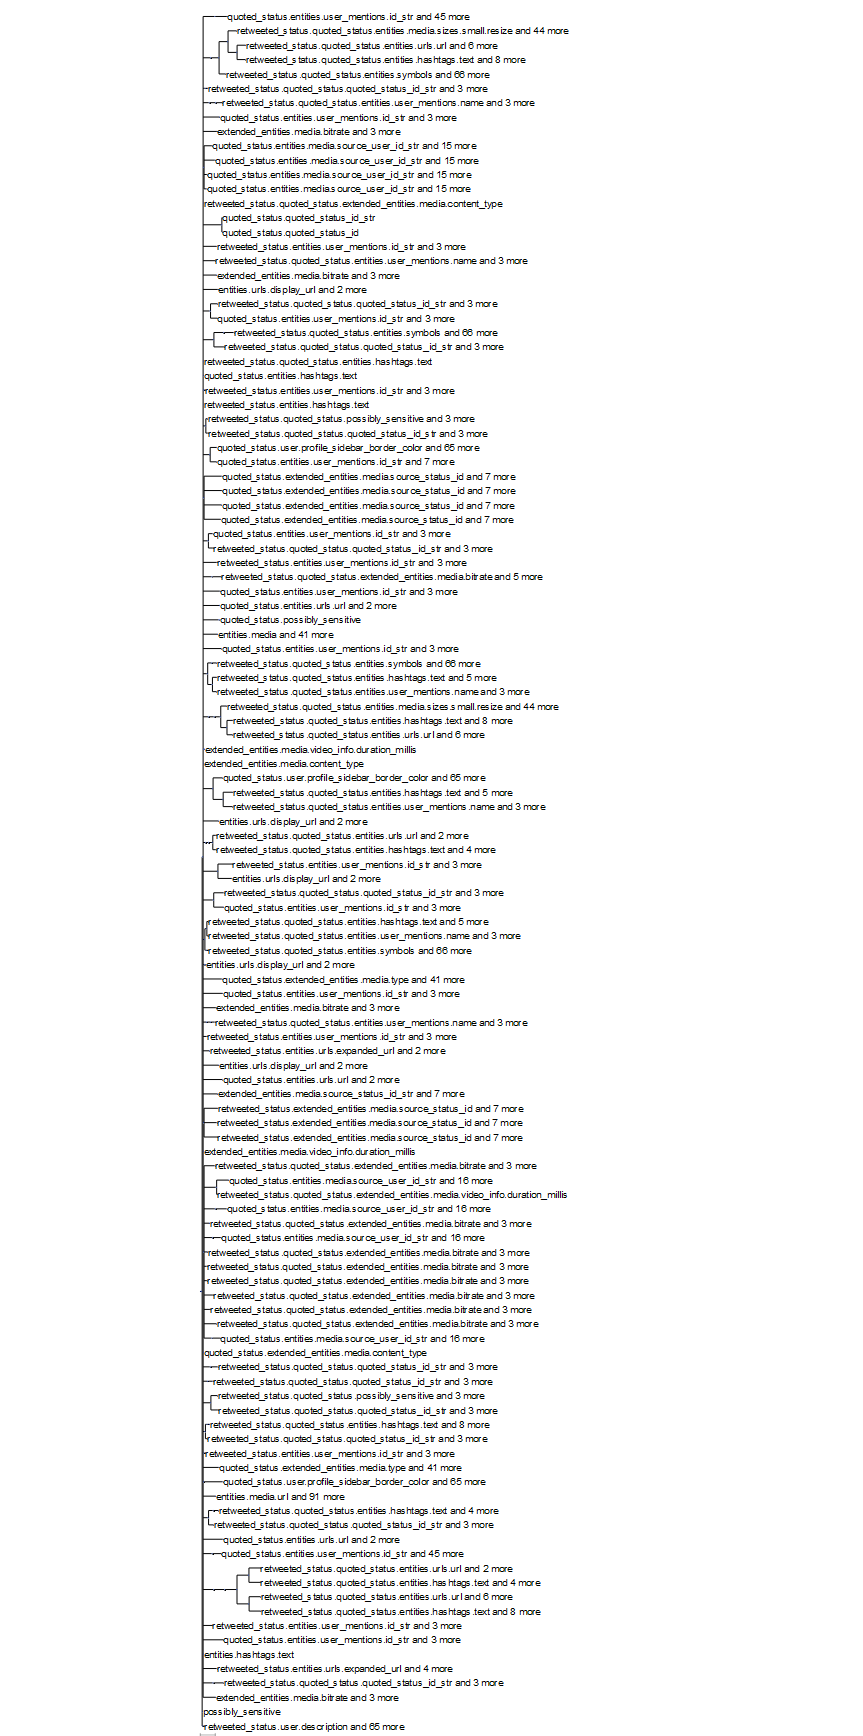
\includegraphics[width=0.57\textwidth]{SchemaSummarization/img/twitterFullTree.png}
    \caption{Without segmentation.}
    \label{fig:seg:twitterFull}
  \end{subfigure}
  \begin{subfigure}{0.59\columnwidth}
    \centering
    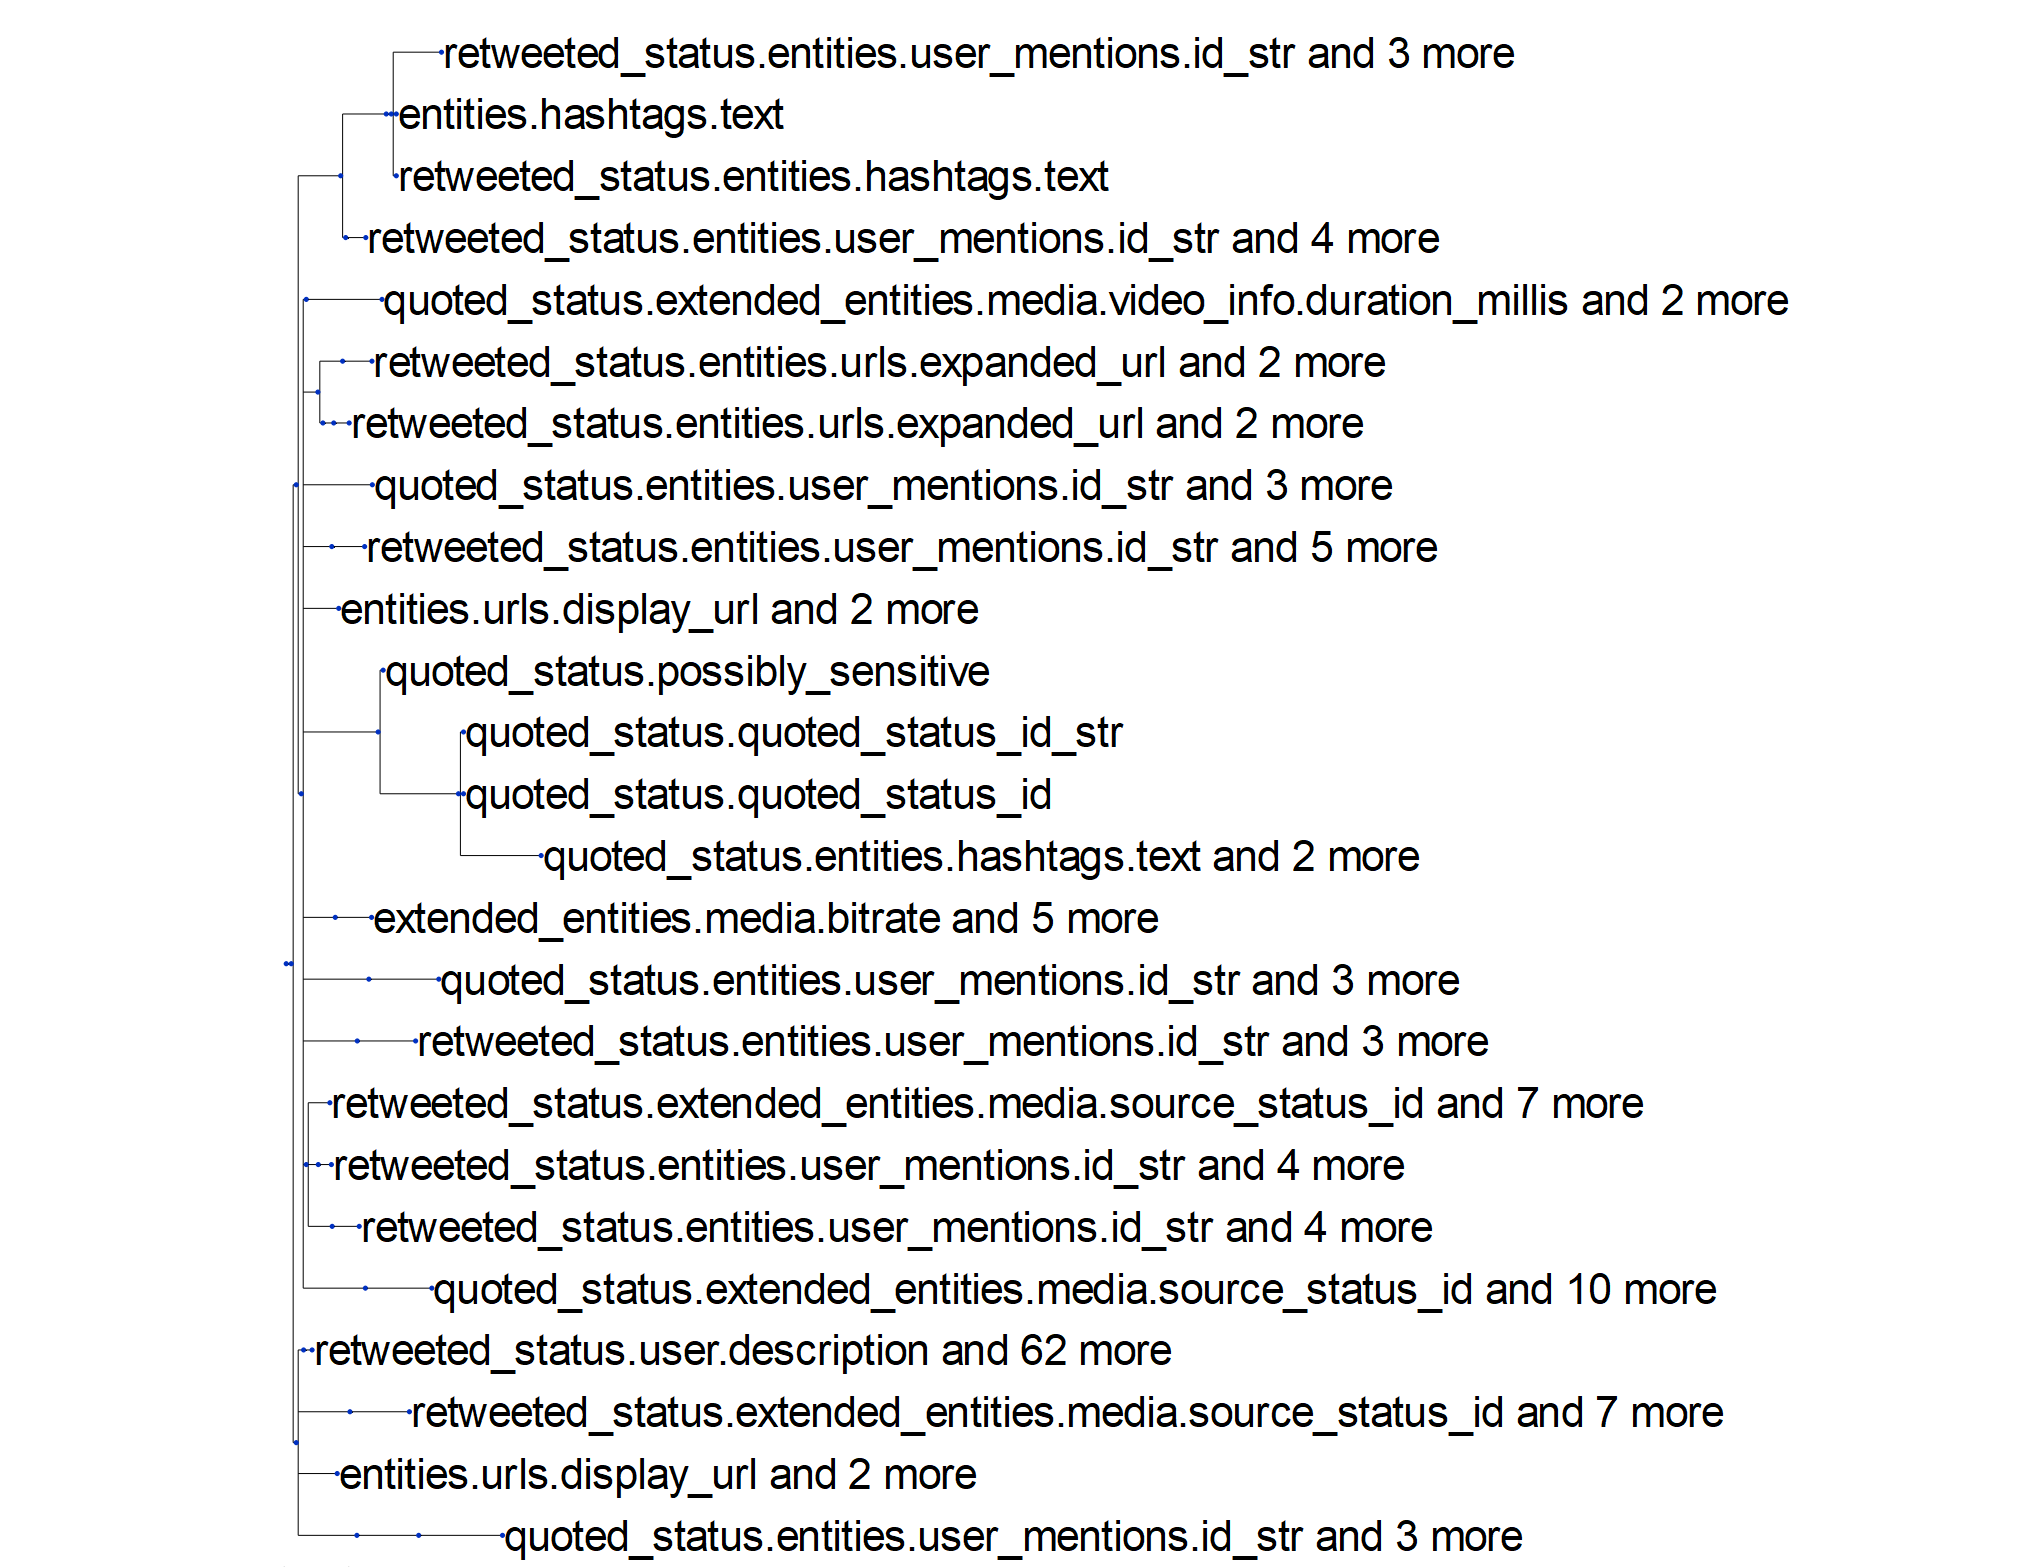
\includegraphics[width=\textwidth]{SchemaSummarization/img/twitterSegment.png}
    \caption{With segmentation.}
    \label{fig:seg:twitterSeg}
  \end{subfigure}
  \caption{Segmentation breaks up schema representations into manageable chunks.}
  \label{fig:seg}
\end{figure}

\subsection{Schema Segmentation}
Specifically, we want to help the user to focus on particular parts of the joint schema;
We want to allow the user to filter out, or segment the schema based on certain required attributes that we call \emph{subschemas}.
We define a subschema $s$ as a set of attributes, where $s$ is contained in one or more source schemas.
Further, the $s$-segment of source schemas $S_1, \ldots, S_N$ to be the subset that contain $s$:
$$\textbf{segment}(s) \defineeq \comprehension{S_i}{i \in [1,N] \wedge s \subseteq S_i}$$
We are specifically interested in visual representations that can help users to identify subschemas of interest.
By then focusing solely on the segments defined by these subschemas can significantly reduce the complexity of the schema design problem, as illustrated in Figure~\ref{fig:seg}.
Figures~\ref{fig:seg:twitterFull} illustrates the full schema summary as a tree, while Figure~\ref{fig:seg:twitterSeg} shows a partial summary identified by the user using the lasso tool we describe shortly.

\begin{figure}[H]
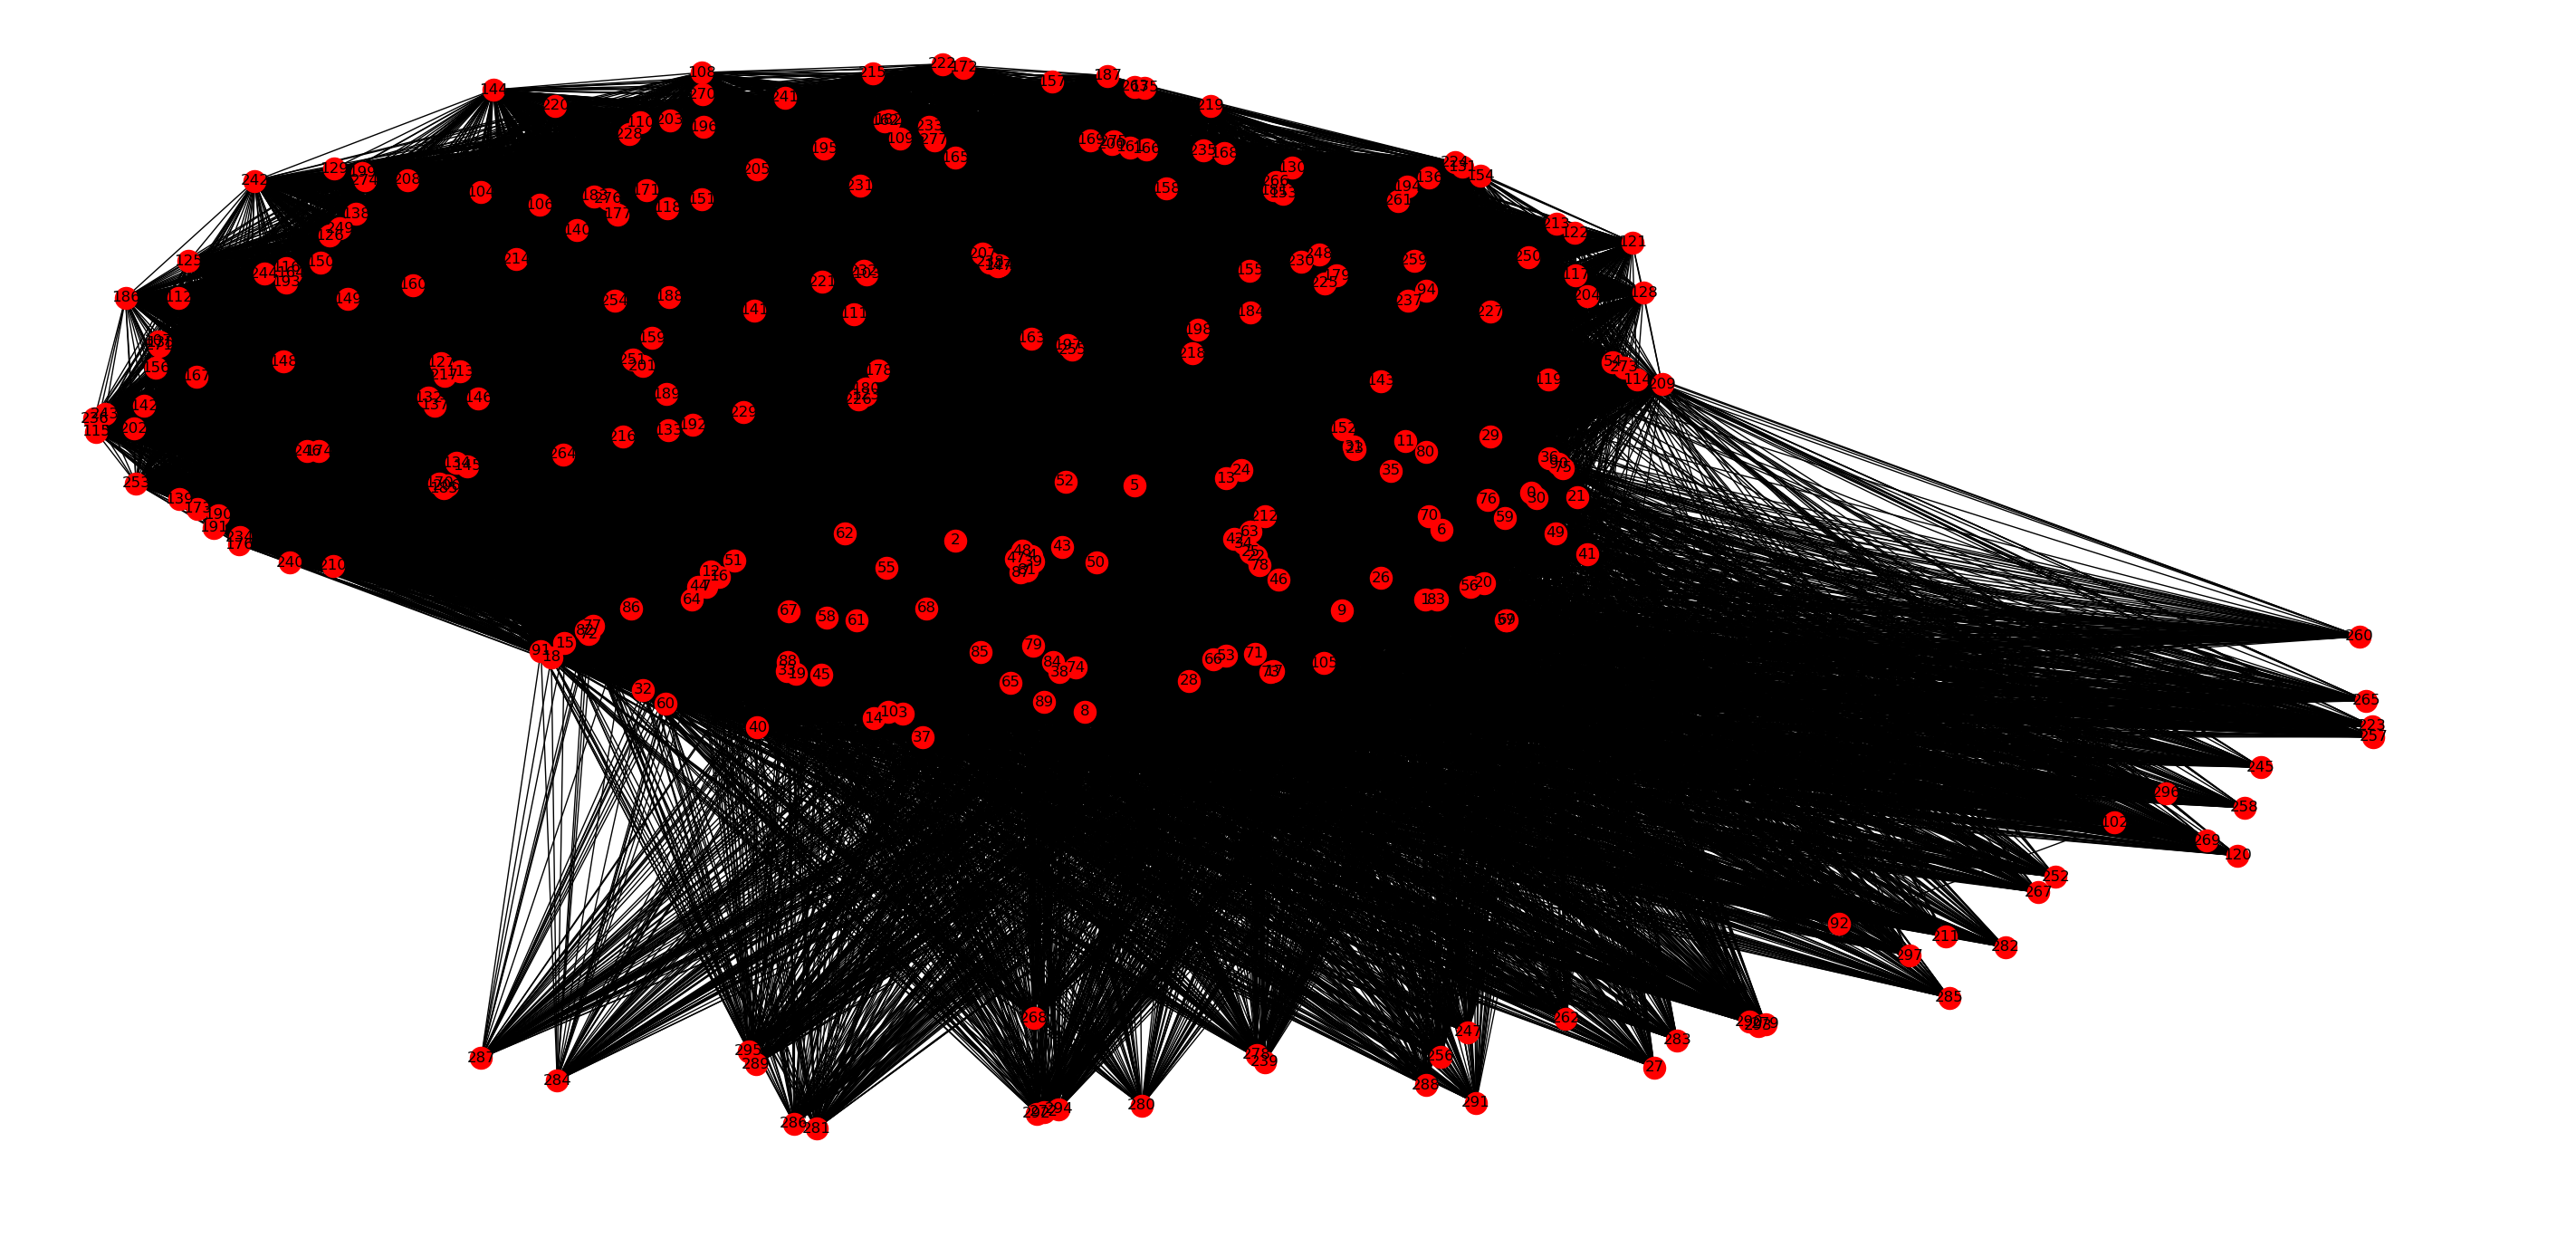
\includegraphics[width=1.0\linewidth]{SchemaSummarization/img/YelpCovMat.png}
\caption{Coveriance Cloud for the full Yelp dataset.}
\label{fig:cloud}
\end{figure}

\tinysection{Covariance Clouds}
Our second visual representation, also like schema summaries, uses correlations and anti-correlations to communicate subschemas of interest.
To generate a covariance cloud, we create a covariance matrix from the source schemas, using the appearance of each attribute as a variable.
Based on a user-controllable threshold, we then construct a graph from the covariance matrix with every attribute as one node, and every covariance exceeding the threshold as an edge.
The graph is then displayed to the user as a cloud using standard force-based layout techniques (e.g., those used by GraphViz~\cite{DBLP:conf/gd/EllsonGKNW00}).  
%\todo{Will: Add figure here}
Cliques in the graph represent commonly co-occurring subschemas that might form segments of interest.  
This includes every conjunctive group identified in the schema summary.
However, unlike the schema summary, this visual representation more effectively captures subschemas with attributes in common.

\tinysection{KNN-PCA Clouds}
While the first visualizaton works on simple schemas, we found that on more complex \json data like Twitter streams~\cite{twitterdecahose}, or the Yelp open dataset~\cite{yelpdata} there were too many inter-attribute relationships, and the resulting visualizatons were noisy.
An approach we settled on is a mixture of Principle Component Analysis (PCA) and K Nearest Neighbor clustering (KNN). 
As before, we treat each source schema as a feature vector with each attribute representing one feature. 
We then use PCA to plot our source schemas in two-dimensions.
The resulting visualization illustrates relationships between source schemas, with greater distances in the visualization representing (approximately) more differences between the schemas.
Hence, clustered groupings of schemas represent potentially interesting sub-schemas.

A key limitation with this visualization is that for more complex datasets the somewhat arbitrary choice of 2 dimensions can be too low.
Conversely adding more dimensions directly through PCA makes the visualization more complicated and hard to follow.
To mitigate these limitations, we use K-Nearest Neighbors (KNN) to colorize the PCA Cloud.
In addition to using PCA, we do KNN clustering on the schemas using a user-provided K (number of clusters).  
Each cluster identified by PCA is assigned a different color.
Combined, these two algorithms to provide users an initial insight into the potential correlations that exist in their dataset.


\begin{figure}
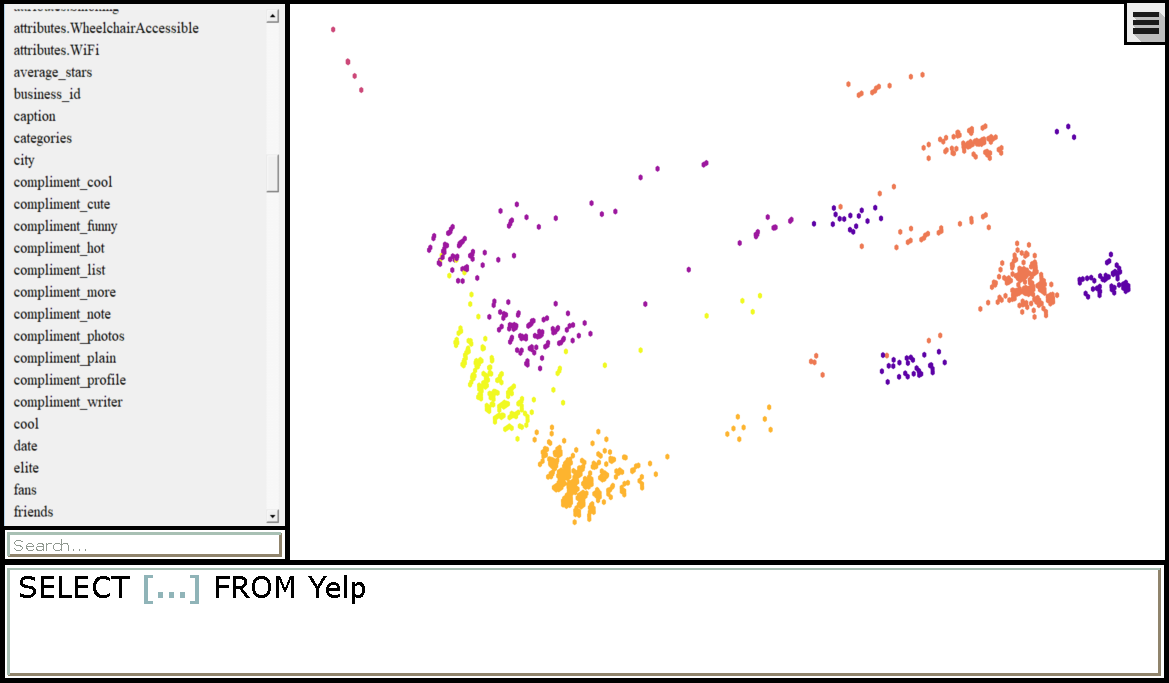
\includegraphics[trim={50mm 25mm 5mm 10mm},clip,width=1.0\linewidth]{SchemaSummarization/img/YelpUI.pdf}
\caption{KNN-PCA cloud with K=6 on the Yelp dataset.}
\label{fig:yelp}
\end{figure}

\begin{example}
Figures~\ref{fig:ui} and \ref{fig:yelp} show an example of the resulting view on Twitter and Yelp data.
Note the much tighter clustering of attributes in the Twitter data: each cluster represents one particular, common type of tweet.
Conversely, the Yelp schema includes a nested collection with, for example, hourly checkins at the business.  
The presence (or absence) of these terminal paths is more variable, and the resulting PCA cloud follows more of a gradient.
\end{example}

These graphs may not initially be intuitive to interpret, but they provide abstract bearings that map directly to phenomenon’s that exist in the data. In lieu of a formal user study, we postulate that the information gained from each algorithm independently will benefit the exploration process that is agnostic to labeled information. This is in contrast to other tools~\cite{Smith:2006:FSS:1187627.1187785}, that largely utilize naming cues and attribute nesting to meet user needs.

\subsection{Schema Exploration}

Now that we have shown the user potentially interesting subschemas, our next task is to help them to (1) narrow down on actually interesting subschemas, and (2) use those schemas to drill down to a segment of the schema data.
For the first step, it is critical that the user develop a good intuition for what the visual representations encode.
One way to accomplish this is to establish a bi-directional mapping between \systemnametwo's two data panes.

To map from visual survey to schema summary, we provide users with a lasso tool.
As illustrated in Figure~\ref{fig:ui}, users can select regions of the KNN-PCA Cloud and the corresponding schemas within that region.  Doing so identifies the maximal subschema contained in all subschemas and regenerates the schema summary pane based only on the segment containing the maximal subschema.  
The maximal subschema itself is also highlighted in the schema summary pane.
On the Covariance cloud, the lasso tool behaves similarly, selecting attributes explicitly rather than a maximal subschema.

The reverse mapping is achieved using highlighting, as illustrated in Figure~\ref{fig:yelpH}.
Users can select one or more attributes (or groupings) in the schema summary pane, and the KNN-PCA Cloud (resp., Covariance Cloud) is modified to highlight schemas in the corresponding segment (resp., to highlight the attributes).
In conjunction with their prior knowledge of their tasks and ideal use cases, we use this approach to perform the initial schema segmentation.

% What patterns immerge and how do we present them
In either case, after selecting a set of attributes or schemas, the analyst may choose to drill down into the selected segment, regenerating both views for the now restricted collection of schemas.
% An analyst may then futher collapse this tree, to produce a view that they can query. Segmentation provides the ability to display tight groups of highly correlated attributes, instead of a large spanning tree that is impossible for a human to process by hand.



% %Attribute co-occurrence can be caused by the presence of an underlying sub-schema and if many co-occur this indicates the presence of a secondary schema, similar to an entity. 
% Segmenting our data first into these entities and then summarizing them, allows us to present the user with features that describe each entity in smaller doses. 
% Additionally, the existence of these entities is derived from insertion methods, and by extension data collection methods, which correspond to natural groupings of attributes that a user expects.


\begin{figure}
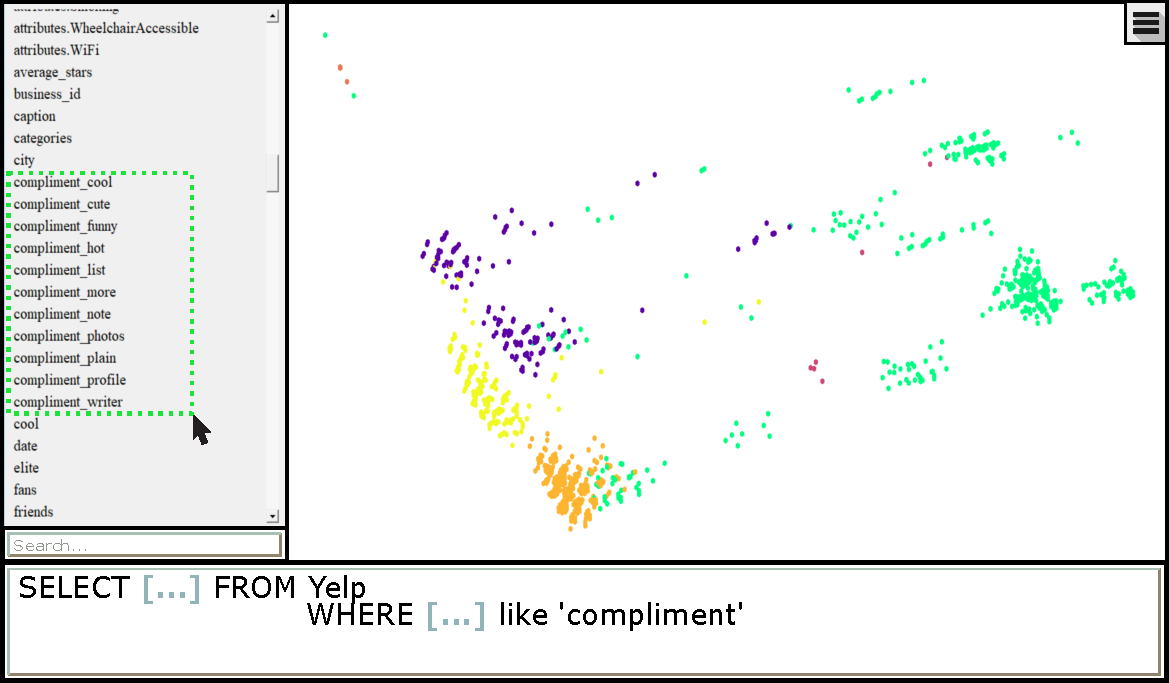
\includegraphics[width=1.0\linewidth]{SchemaSummarization/img/YelpUIH.pdf}
\caption{Points containing user selected attributes are highlighted green.}
\label{fig:yelpH}
\end{figure}


%\begin{itemize}
%\item cov matrix clique issues
%\item knn limitations
%\item PCA limitations and benefits
%\item goal is to first reduce the 
%\end{itemize}

%Through our user interface groups of attributes may be highlighted, this then feeds back into our PCA plot to highlight the points that these attributes are present in. 
%If this group of attributes has high co-occurrence, then they are likely to appear grouped and ideally leads the user to other attributes that also co-occur and are of significance.

\subsection{An Iterative Approach}
At any time in our exploration pipeline analysts may stop where they are, take the knowledge they gained about their dataset, and restart the process from the beginning. 
Through exploring the Twitter dataset we found retweets and quoted tweets to have a high correlation, with this knowledge we can then start back at the beginning and depending on whether our task allows us to merge these attributes, we can then choose a more appropriate K value for KNN. 
In addition, attributes that have no relationship to core attributes, such as a users profile\_image\_url being present, can easily be pruned to compress our summary output. 
By incrementally learning about their dataset, an analyst can converge on the views required for their tasks.


%Will: How does the data get summarized for user consumption. 
%Some UI sketches/screenshots would be appropriate.
%\begin{itemize}
%\item The schema is presented to the user
%\item The user is then shown a 2-dimensional representation of their data using PCA
%\item Iteratively use a generic clustering algorithm to help detect clusters and relationships in their data
%\item Select a subregion of the map to expore relaitonships that exist and what each group represents
%\item |eigenVector| x norm($\sum\nolimits $multiplicity x featureVector), this results in a score for each column that is based on occurance and variation
%\item the higher this score, the more 'representative' of the cluster this feature is
%\item Iterate through this process to determine what the defining characteristics of each group is, and how it relates to other groups
%\end{itemize}


